\documentclass[11pt,a4paper]{article}
\usepackage[margin=1in]{geometry}
\usepackage{booktabs,graphicx,float,hyperref,amsmath}
\usepackage[default]{sourcesanspro}
\title{MNIST Generative Modeling and Latent-Space Exploration\\\large A Controlled $\beta$-VAE Trade-off Study}
\author{Mohammad Torabi \\ 404422041}
\date{Course: Data Mining \\ Instructor: Dr. Hadi Farahani \\ August 2026}
\begin{document}
\maketitle
\begin{abstract}
In this project, I train two-dimensional variational autoencoders on MNIST digits. My contribution is a controlled $\beta\in\{0.5,1,4\}$ study of the reconstruction--regularization trade-off. The saved test results show that $\beta=0.5$ has the best reconstruction BCE (137.98) and the best ELBO (141.70). As $\beta$ increases, KL decreases from 7.43 to 4.37, while reconstruction BCE becomes worse from 137.98 to 143.57. This is the expected trade-off, but the 2-D latent space is deliberately restrictive.
\end{abstract}

\section{Problem, Data, and Method}
MNIST contains 60,000 training digit images and 10,000 test images of size $28\times28$. I use a fixed 55,000/5,000 training/validation split and keep the 10,000 test images for evaluation. The encoder is an MLP that outputs $\mu$ and $\log\sigma^2$ for a two-dimensional Gaussian posterior. The decoder maps a reparameterized latent sample back to pixel probabilities.

The loss is
\[
\mathrm{BCE}(x,\hat{x})+\beta D_{KL}(q_\phi(z|x)\Vert\mathcal{N}(0,I)).
\]
I keep the architecture, seed, optimizer, batch size, and early stopping settings fixed across the three $\beta$ values. I report reconstruction BCE, KL, ELBO, 15-nearest-neighbor accuracy on latent means, and generated-image diversity. This makes the experiment more than only showing visually appealing samples.

\section{Real Results and Latent Structure}
The test results in Table~\ref{tab:results} come from the saved artifacts. The smaller regularization value, $\beta=0.5$, gives the best reconstruction BCE (137.98), best ELBO (141.70), and highest k-NN accuracy (0.772, only slightly above 0.771 for $\beta=4$). Increasing $\beta$ from 0.5 to 4 lowers KL from 7.43 to 4.37. At the same time, reconstruction BCE increases by 5.59 and ELBO increases by 19.37, which means the reconstructions become less accurate under this loss definition.

The diversity score increases from 5.73 at $\beta=0.5$ to 6.09 at $\beta=4$. I treat this carefully: pairwise pixel diversity is not the same as perceptual sample quality or disentanglement. It only gives one quantitative signal that the generated images vary more.

\begin{table}[H]\centering
\caption{Saved held-out test metrics for the matched $\beta$ sweep.}\label{tab:results}
\input{generated_results.tex}
\end{table}
\input{generated_summary.tex}
\begin{figure}[H]\centering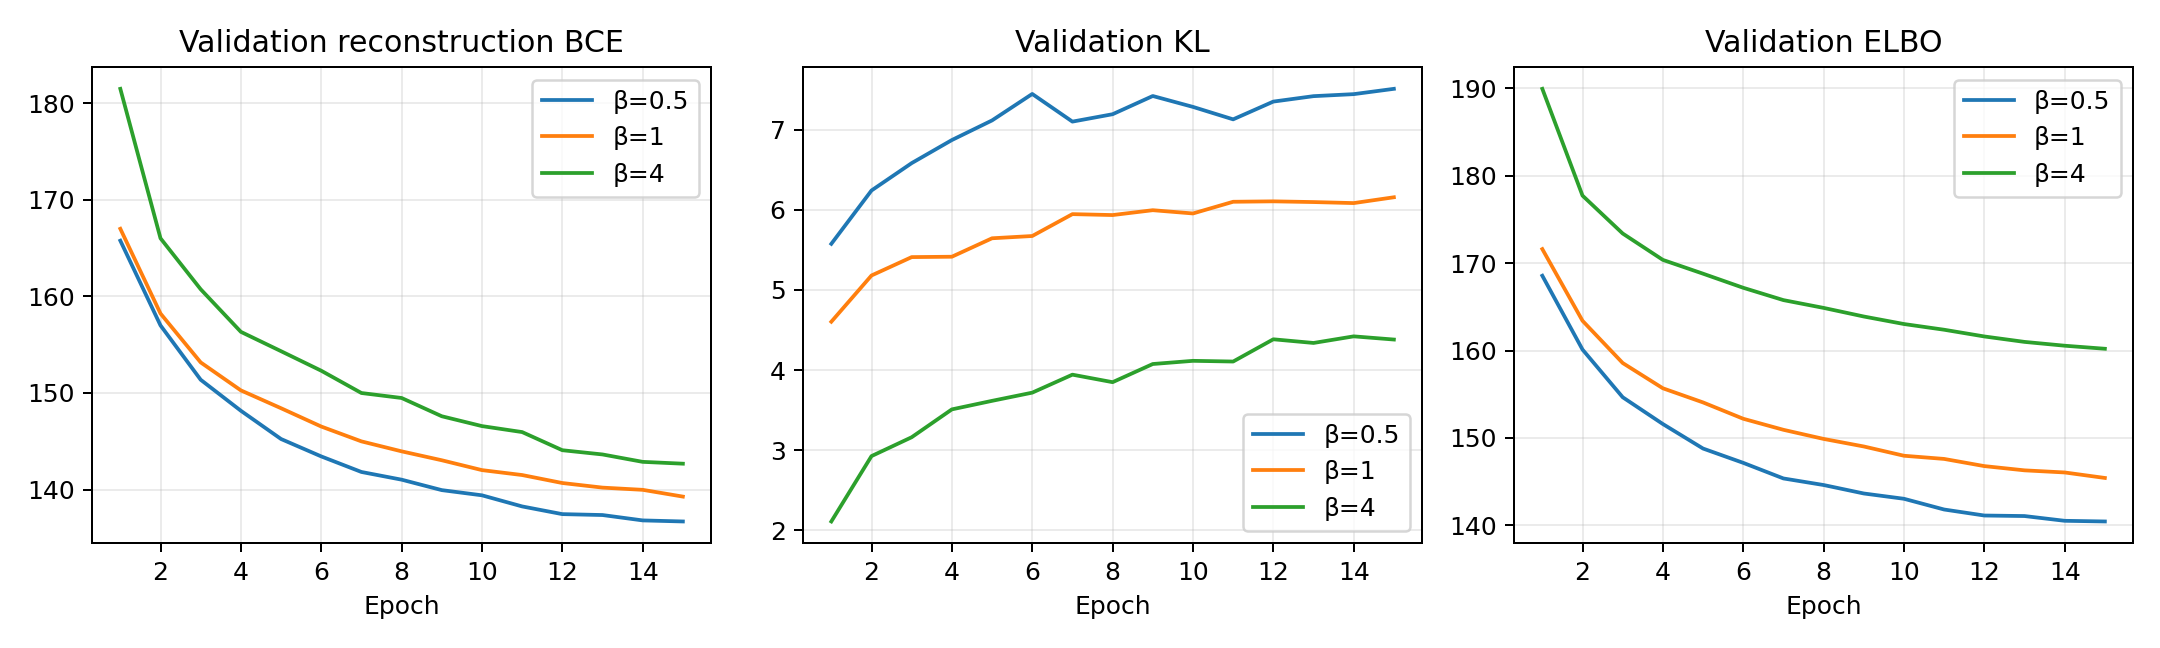
\includegraphics[width=\linewidth]{figures/elbo_curves.png}\caption{Validation reconstruction BCE, KL, and ELBO during training.}\label{fig:curves}\end{figure}
\begin{figure}[H]\centering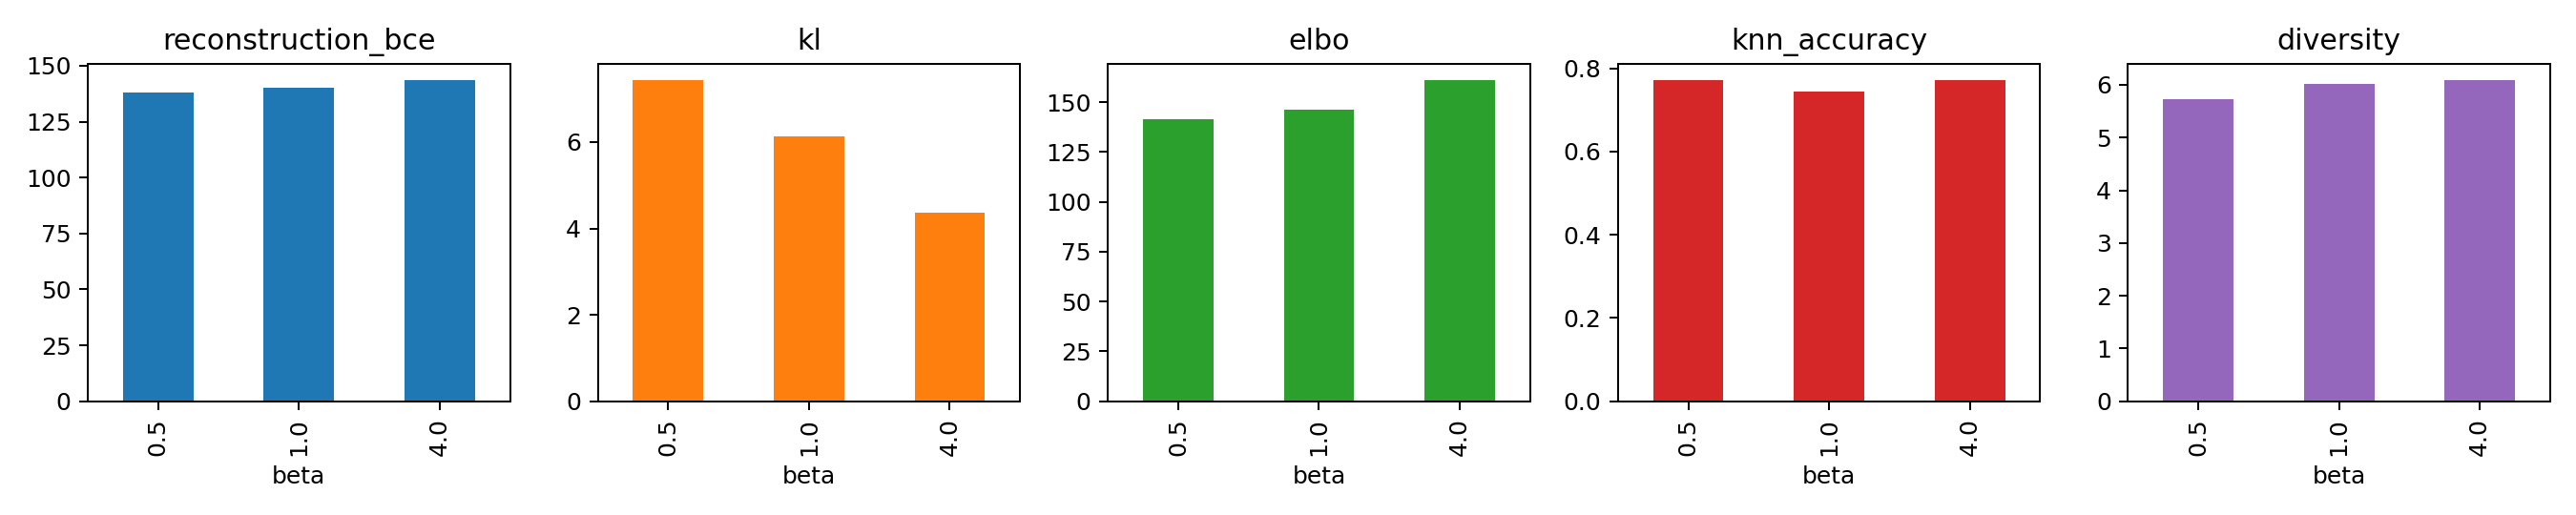
\includegraphics[width=\linewidth]{figures/metric_tradeoff.png}\caption{Quantitative reconstruction--regularization trade-off.}\label{fig:tradeoff}\end{figure}
\begin{figure}[H]\centering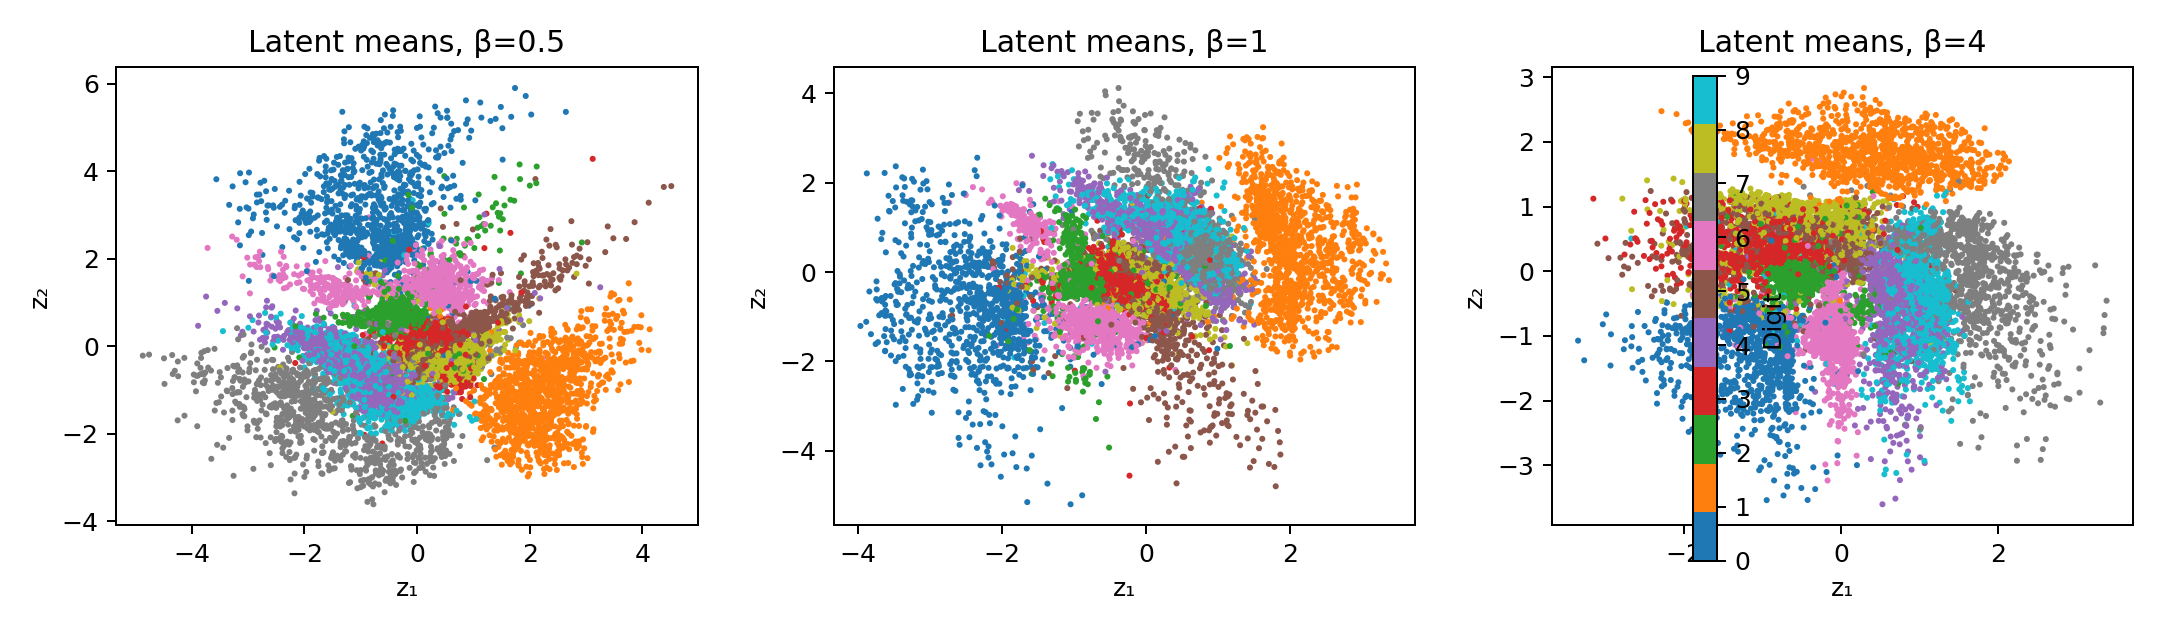
\includegraphics[width=\linewidth]{figures/latent_scatter.png}\caption{Test-digit latent means for each $\beta$ value.}\label{fig:scatter}\end{figure}

\section{Generation and Interpolation}
The saved figures include random prior samples, reconstructions, interpolation between two test latent means, and a regular latent grid. They are useful qualitative checks that the decoder receives a continuous two-dimensional latent space. However, the digits are limited by the small latent dimension, so fine details should not be expected.
\begin{figure}[H]\centering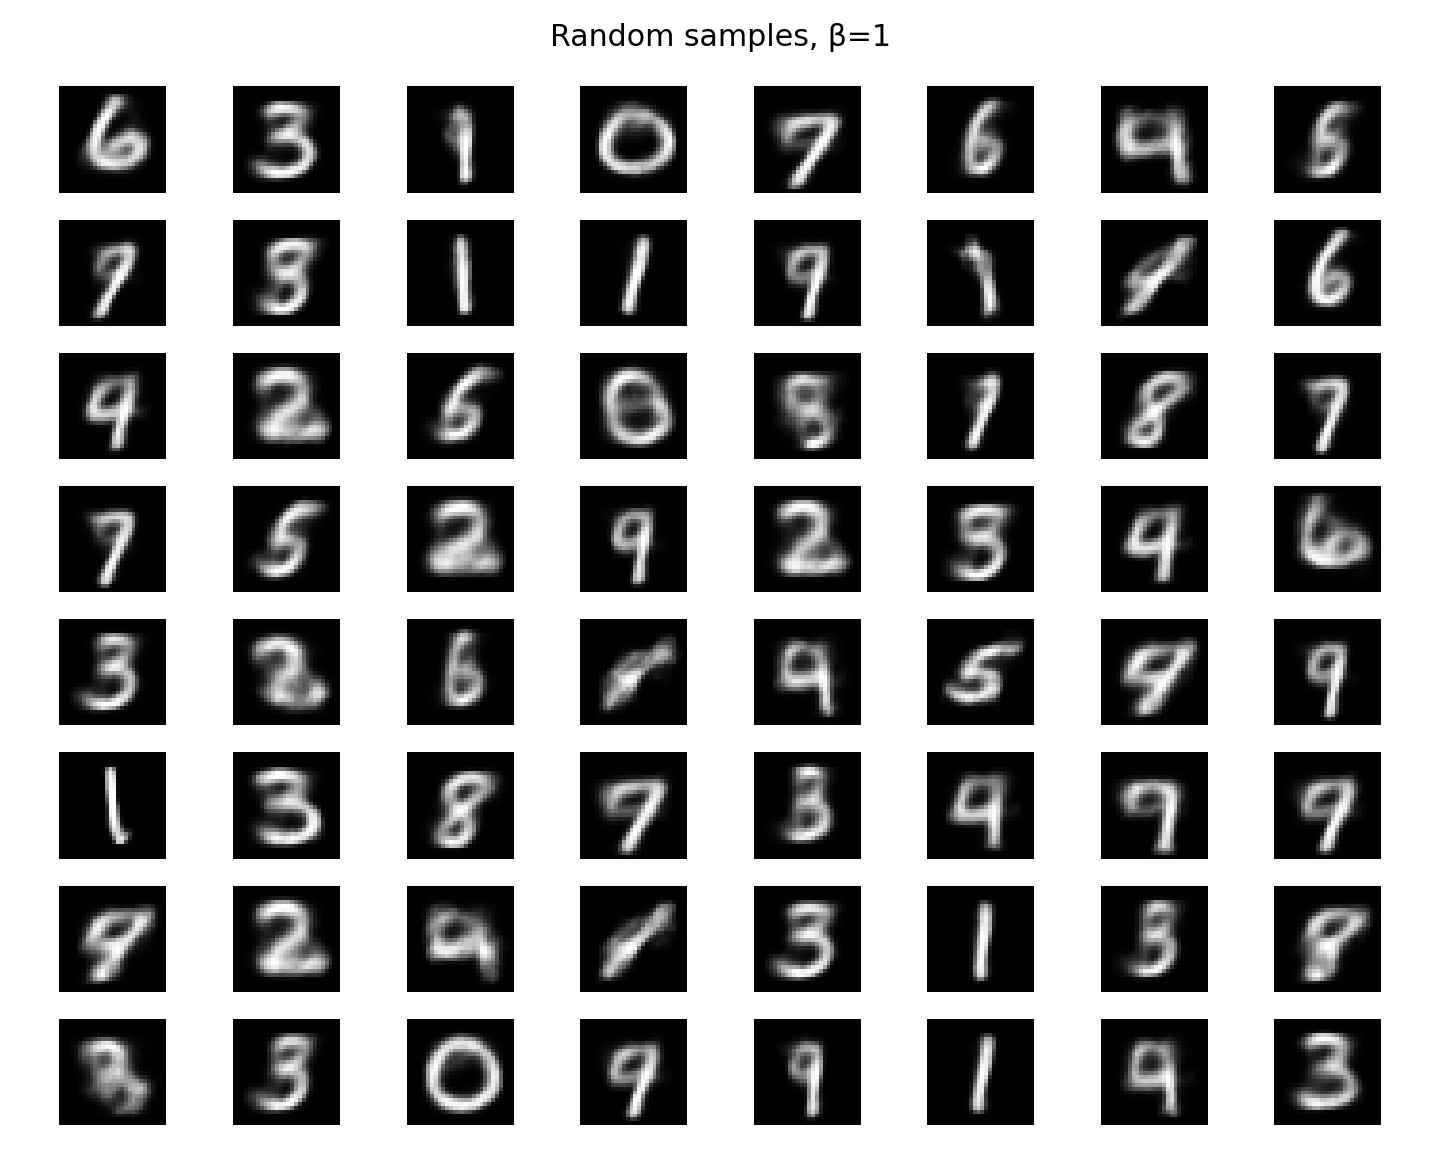
\includegraphics[width=.82\linewidth]{figures/samples_beta_1.png}\caption{Random prior samples for $\beta=1$.}\label{fig:samples}\end{figure}
\begin{figure}[H]\centering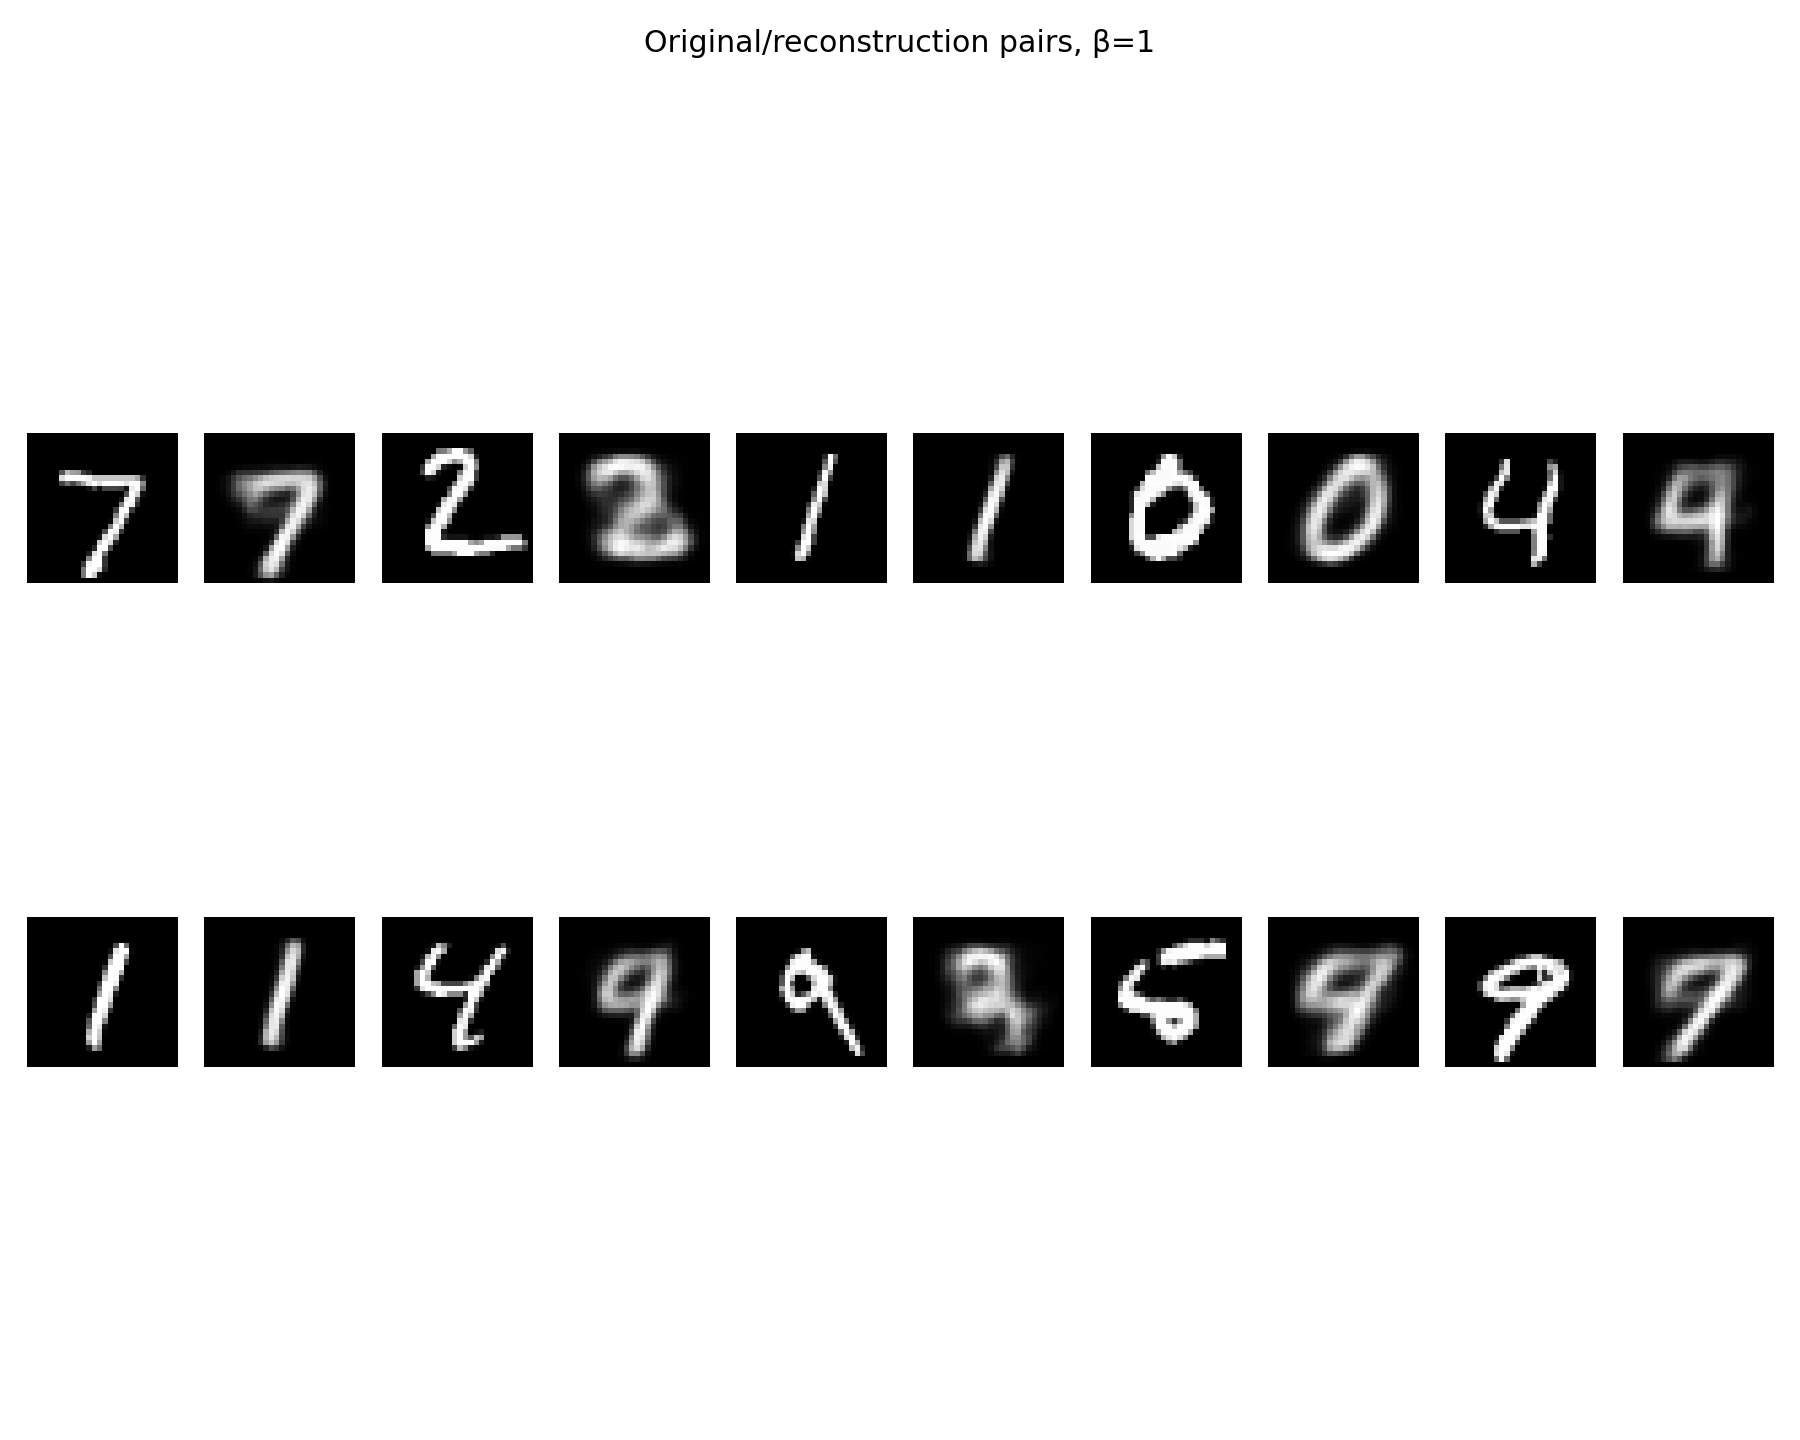
\includegraphics[width=\linewidth]{figures/recon_beta_1.png}\caption{Original digits and reconstructions for $\beta=1$.}\label{fig:recon}\end{figure}
\begin{figure}[H]\centering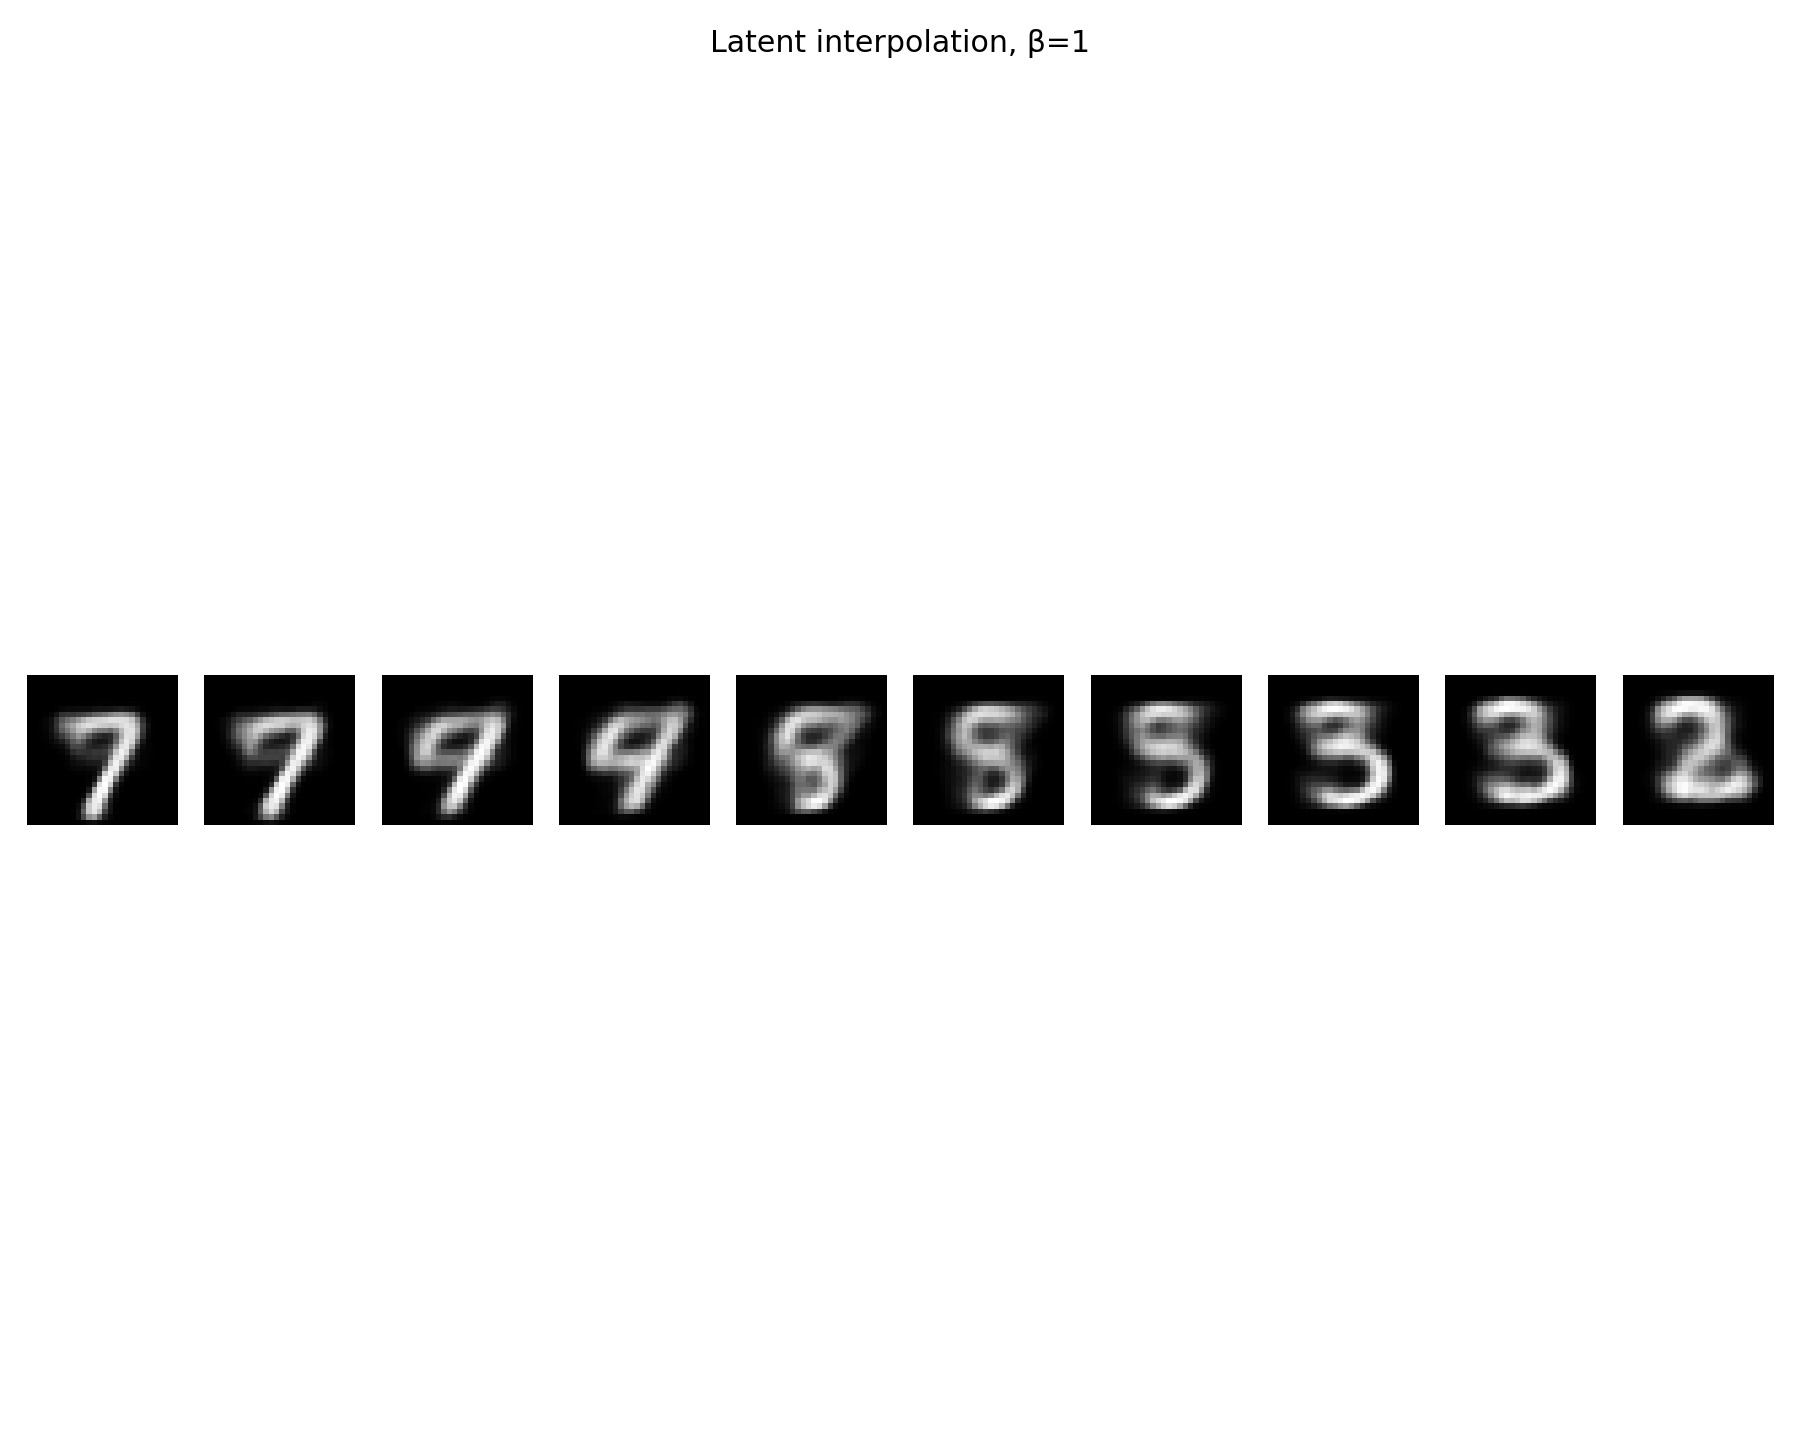
\includegraphics[width=\linewidth]{figures/interpolation.png}\caption{Decoded linear interpolation between two test examples.}\label{fig:interpolation}\end{figure}
\begin{figure}[H]\centering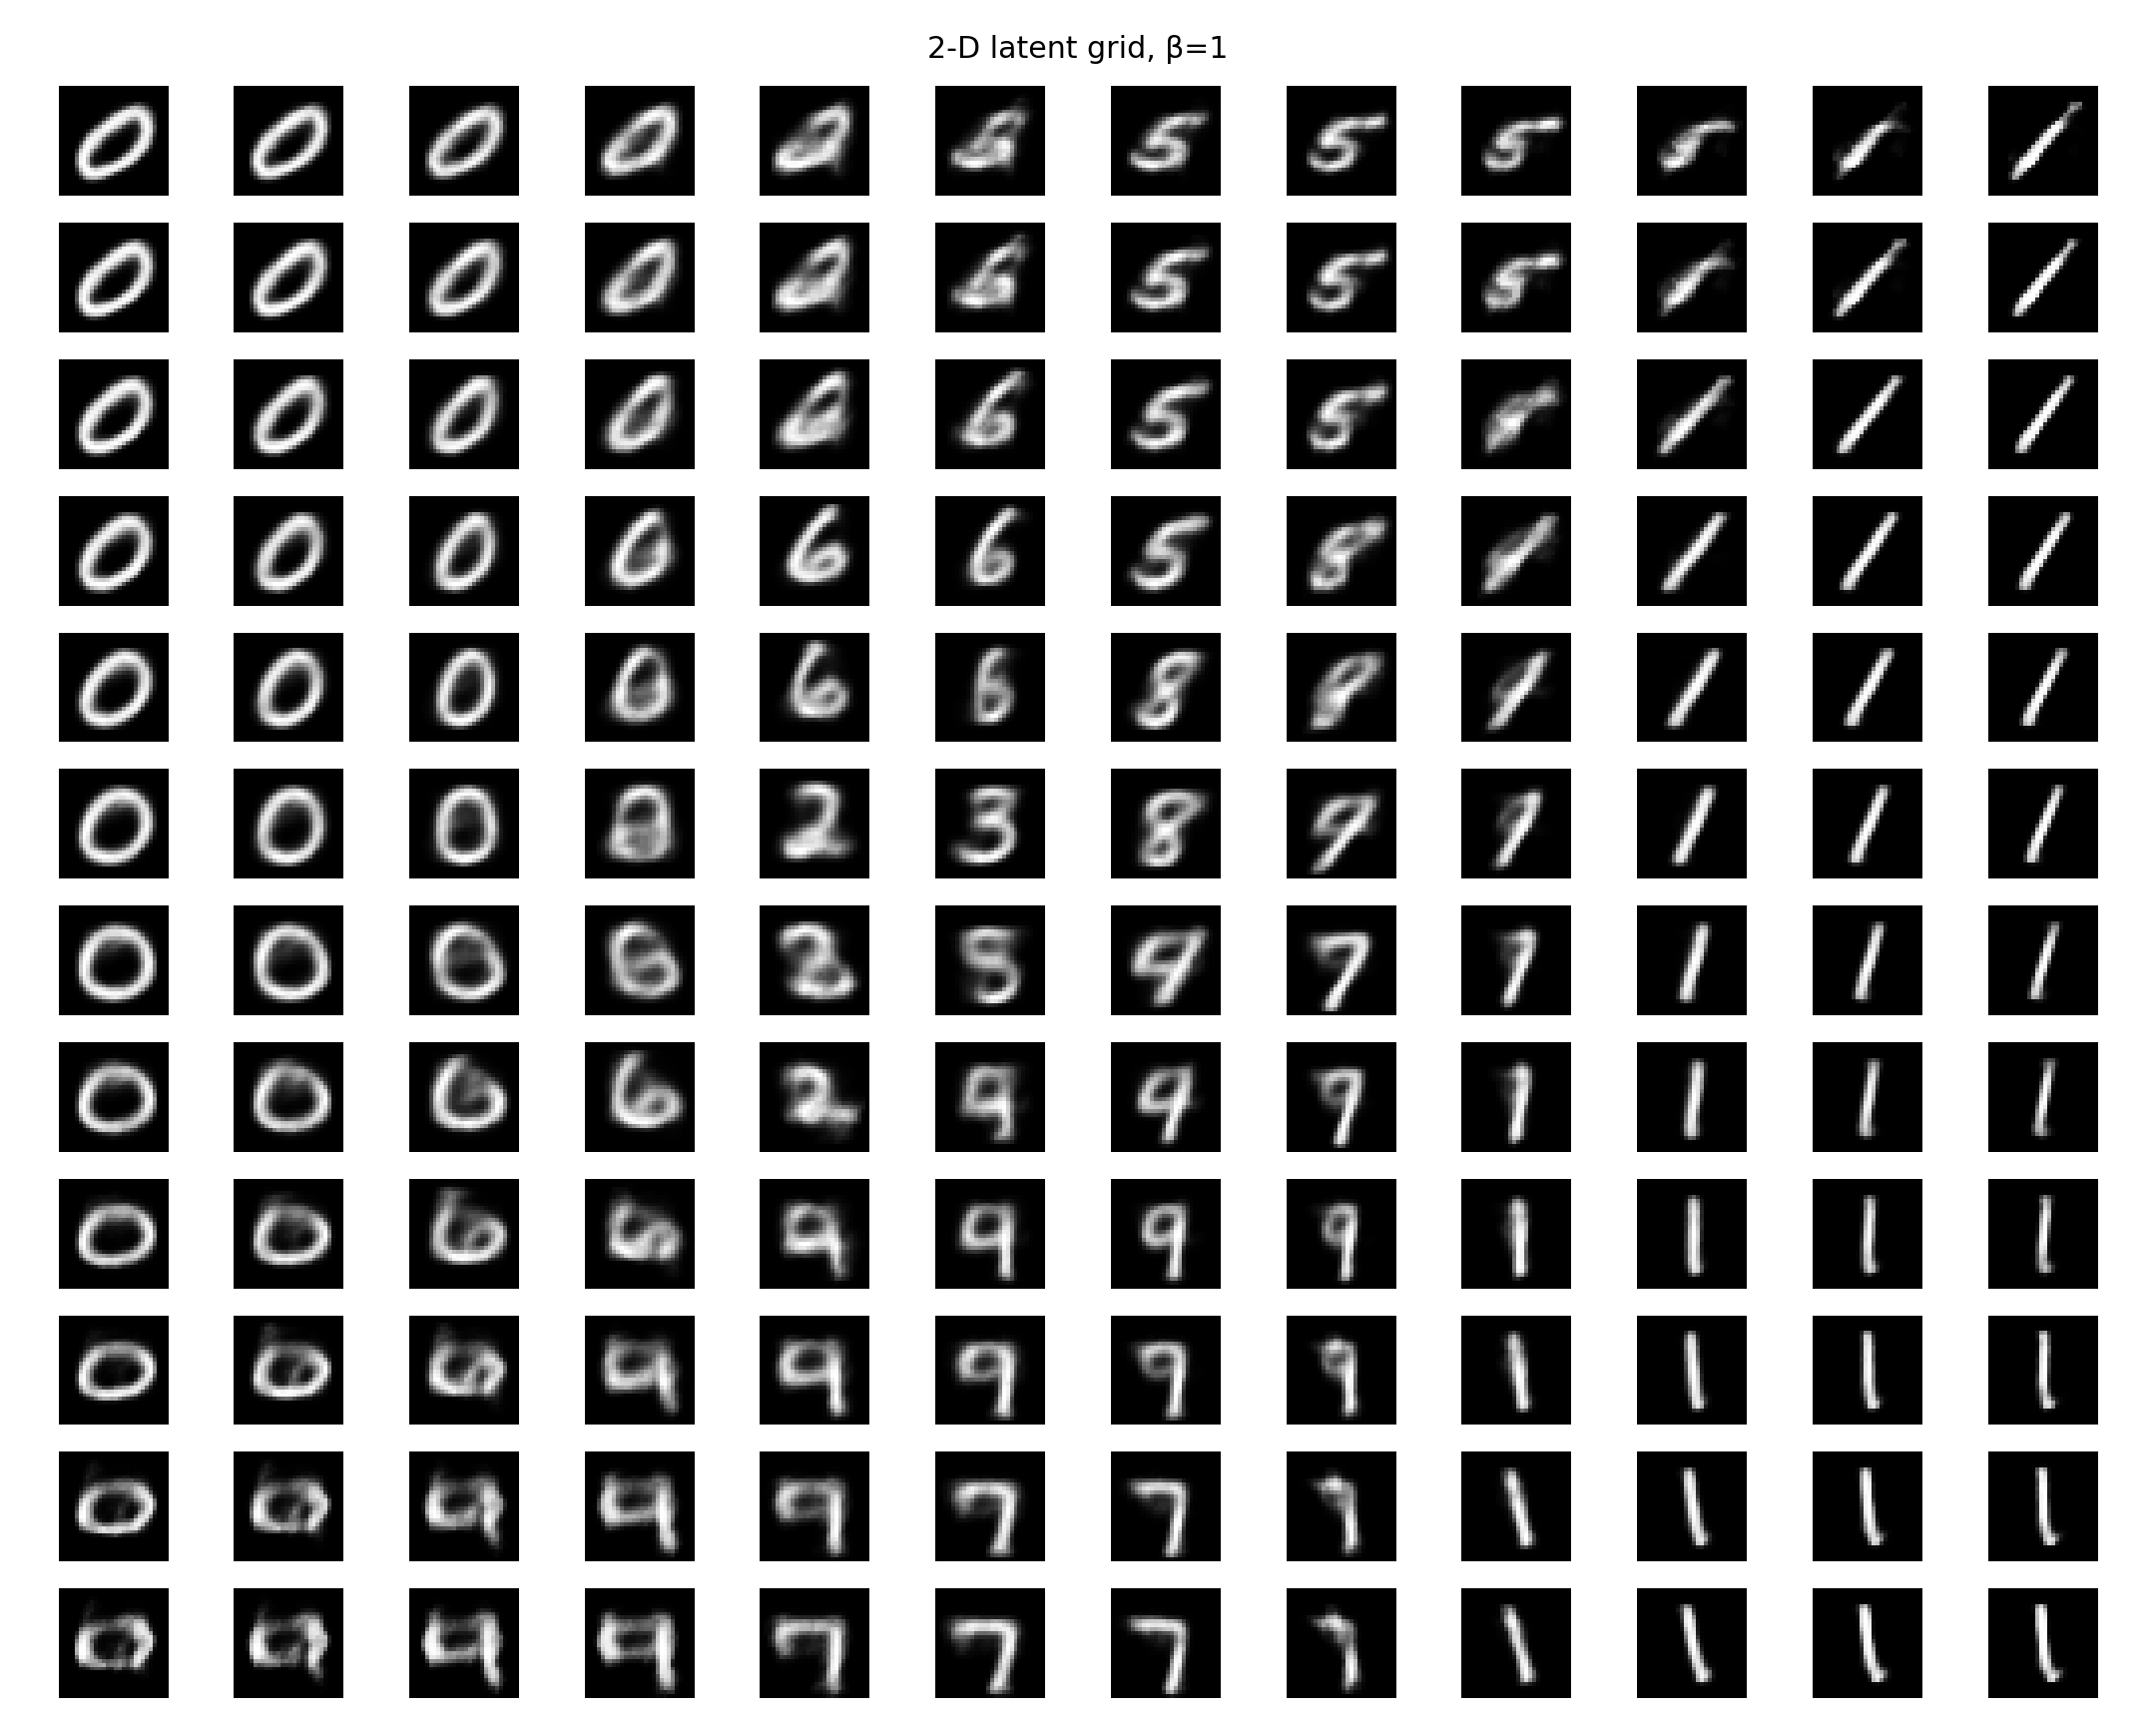
\includegraphics[width=\linewidth]{figures/latent_grid.png}\caption{A grid decoded from the standard-normal latent plane.}\label{fig:grid}\end{figure}

\section{Discussion and Observation}
\subsection*{Why are VAE interpolations smoother?}
The KL term encourages the posterior of each digit to stay close to a common Gaussian prior. Therefore, nearby latent positions are more likely to have meaningful decoder outputs. A line between two encodings can stay in a region where the decoder was trained to work. A plain autoencoder has no such pressure, so empty or irregular latent regions can make interpolation less useful. The cost is that the latent code cannot store unlimited reconstruction information.

\subsection*{What if the prior changed?}
A mixture prior could give different digit modes separate latent regions and may create sharper samples if the inference model can match it. But it makes mode assignment and optimization harder. A uniform-ball prior changes the geometry and boundary behavior; the Gaussian encoder and decoder design would need to change together. I would not assume that changing the prior automatically improves the results.

\section{Limitations and Reproducibility}
This experiment evaluates a real full 55,000-image training split and 10,000-image test split, but it is still a simple MLP VAE with only two latent dimensions. Pixel diversity and k-NN accuracy do not directly measure sample realism or disentanglement. Future work could add a disentanglement metric, a perceptual sample-quality metric, or latent traversals designed for specific digit attributes. Run \path{python scripts/train.py}, then \path{python scripts/build_report_assets.py}, to recreate the saved artifacts and report figures.
\end{document}
